%!TEX program=xelatex

\documentclass[12pt,a4paper,UTF8]{article}
\usepackage[fontset=fandol]{ctex} % Chinese support, using Fandol fonts
\usepackage{graphicx} % Insert images
\usepackage{listings} % Print source code
\usepackage{color} % Color support
\usepackage{booktabs} % Professional table support
\usepackage{pdflscape} % Landscape pages support in PDF
\usepackage[colorlinks,linkcolor=blue]{hyperref}
\usepackage{background}

% Customize hyperref format (it's set to no special format here)
\hypersetup{hidelinks}

% Declare directories to search for graphics files for graphicx
\graphicspath{{figures/}{logo/}}

% 自定义代码块样式
\lstset
{
    language=C++,
    basicstyle=\ttfamily\footnotesize,
    keywordstyle=\bfseries\color[rgb]{0, 0, 1},
    identifierstyle=\color[rgb]{0.5, 0.3, 0.1},
    stringstyle=\color[rgb]{0.6, 0.1, 0.1},
    commentstyle=\itshape\color[rgb]{0.05, 0.5, 0.05},
    backgroundcolor=\color[gray]{0.95},
    numbers=left,
    numbersep=5pt,
    numberstyle=\color[gray]{0.6},
    breaklines=true
} 

% Define source code style for listings
\lstdefinestyle{cpp-style}{
    language=C++,
    basicstyle=\ttfamily\footnotesize,
    keywordstyle=\bfseries\color[rgb]{0, 0, 1},
    identifierstyle=\color[rgb]{0.5, 0.3, 0.1},
    stringstyle=\color[rgb]{0.6, 0.1, 0.1},
    commentstyle=\itshape\color[rgb]{0.05, 0.5, 0.05},
    backgroundcolor=\color[gray]{0.95},
    numbers=left,
    numbersep=5pt,
    numberstyle=\color[gray]{0.6},
    breaklines=true
}

% Define new command for title page
\newcommand{\reporttitle}[2]{
    \LARGE\textsf{#1}\quad\underline{\makebox[12em]{#2}}
}
\newcommand{\reportinfo}[2]{
    \large\makebox[4em]{\textsf{#1}}\quad\underline{\makebox[18em]{#2}}
}

% The document begins here
\begin{document}
    %Background settings
    \backgroundsetup{scale=2,angle=0,opacity=0.5,pages='some',contents={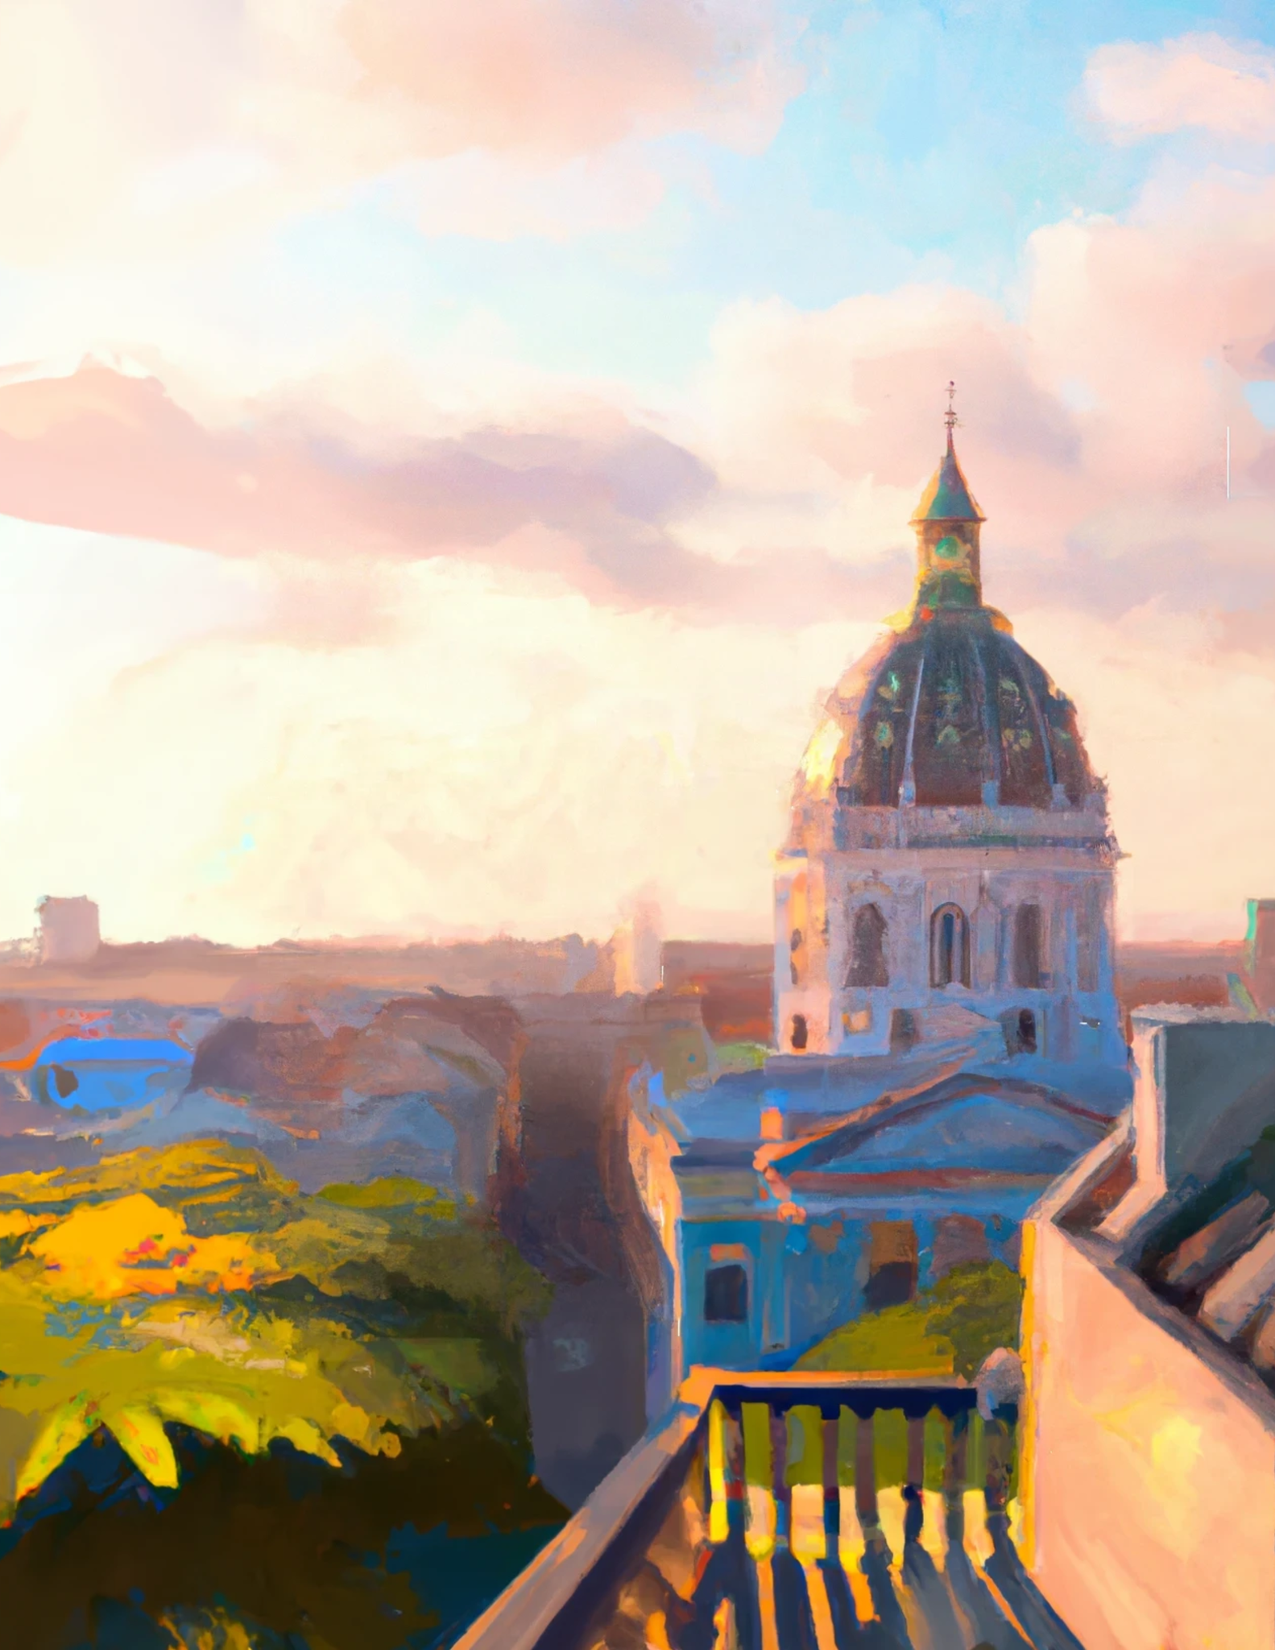
\includegraphics[width=\paperwidth,height=\paperwidth,keepaspectratio]{pictures/background.png}}}

    \begin{titlepage}
        \centering
        \vspace*{\fill}    
        \BgThispage
        {\huge\textsf{实\ 验\ 报\ 告}}\\[48pt]
        \reporttitle{实验名称}{Python}\\[72pt]
        \reportinfo{课程名称}{系统开发工具基础}\\[8pt]
        \reportinfo{学\hspace{\fill}号}{23070001092}\\[8pt]
        \reportinfo{学生姓名}{王佳晖}\\[8pt]
        \reportinfo{实验日期}{2024年9月6日}\\
        \href{https://github.com/JOINKINGER/TheSecondExperiment}{个人LaTex模版github链接}
        (https://github.com/JOINKINGER/TheSecondExperiment)
        \vspace*{\fill}
    \end{titlepage}

    \tableofcontents
    \newpage

    \NoBgThispage
    \section{实验目的}
    \begin{enumerate}    
        \item 熟悉Python基本数据类型:包括数字、字符串、列表、元组、字典和集合等。
        \item 掌握Python的控制结构:理解并使用if语句、循环(for和while)等基本控制语句。
        \item 学习Python的函数与模块的使用:学习函数的定义、调用,以及如何使用Python模块。
        \item 学习并练习Python在视觉中的应用。
    \end{enumerate}
    
    \section{实验内容}
    \subsection{Python基本语法}
    \begin{enumerate}
        \item \textcolor{blue}{变量定义}\\
        注:Python定义变量时不用指定变量类型\\
        \textcolor{blue}{用法如下}\\
        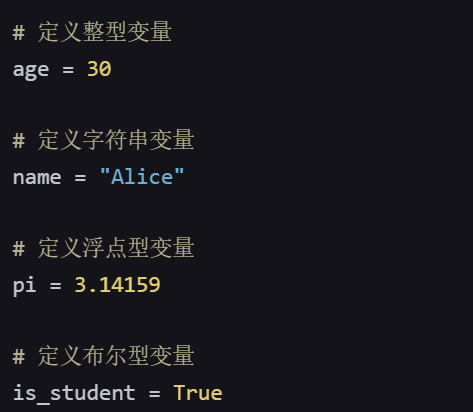
\includegraphics[scale=0.5]{pictures/2.png}
        \item \textcolor{blue}{变量类型}\\
        整型(Integer):用于表示整数,可以是正数或负数。\\
        浮点型(Float):用于表示带有小数点的数,即实数。\\
        字符串(String):用于表示文本数据,由字符组成,用引号(单引号'或双引号")括起来。\\
        列表(List):用于存储一系列有序的项目,项目可以是不同类型的数据。列表是可变的,意味着你可以添加、删除或修改列表中的项目。\\
        元组(Tuple):与列表类似,但元组是不可变的,一旦创建就不能修改。\\
        字典(Dictionary):用于存储键值对,其中每个键都映射到一个值。字典是可变的,但你不能修改键,只能修改与键关联的值。\\
        集合(Set):一个无序的、不包含重复元素的集合。集合主要用于数学上的集合操作,如并集、交集、差集和对称差集。\\
        布尔型(Boolean):只有两个值,True 和 False,用于表示逻辑条件。\\
        \textcolor{blue}{用法如下}\\
        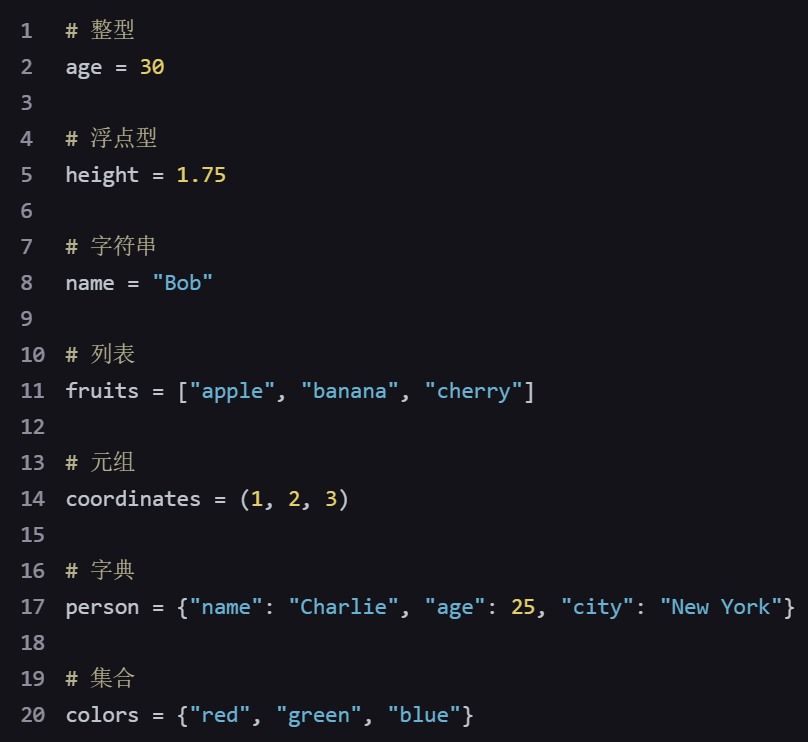
\includegraphics[scale=0.4]{pictures/1.png}\\[8pt]
        \textcolor{red}{注:可以用type()函数检查变量类型}\\
        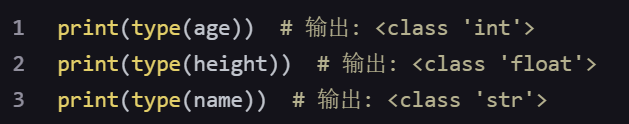
\includegraphics[scale=0.5]{pictures/3.png}
        \item \textcolor{blue}{运算符与表达式}\\
        Python中的运算符与表达式,包括算术运算符、比较运算符、逻辑运算符、赋值运算符、位运算符以及成员运算符\\
        部分特殊的运算符如下:\\
        /:除法(结果为浮点数)\\
        //:整数除法(结果为商的整数部分)\\
        **:幂运算(左操作数的右操作数次幂)\\
        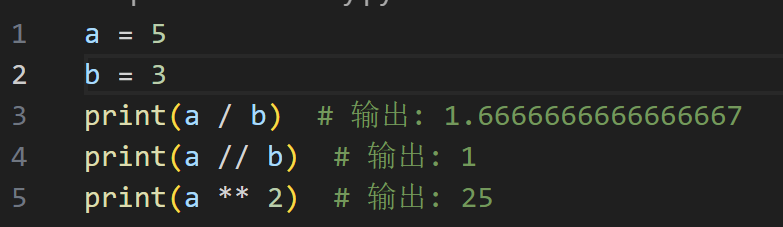
\includegraphics[scale=0.5]{pictures/4.png}\\
        and:逻辑与(两个条件都为True时返回True)\\
        or:逻辑或(至少一个条件为True时返回True)\\
        not:逻辑非(条件为True时返回False,为False时返回True)\\
        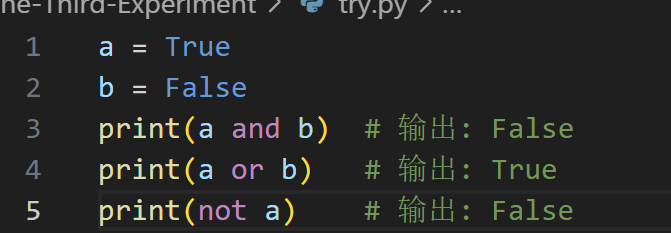
\includegraphics[scale=0.5]{pictures/5.png}\\
        in:如果成员在序列中,返回True\\
        not in:如果成员不在序列中,返回True\\
        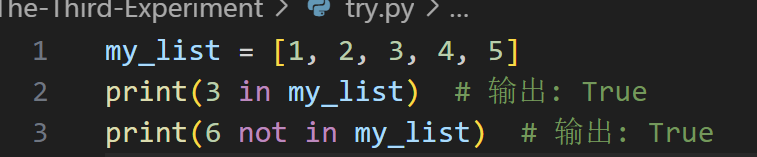
\includegraphics[scale=0.5]{pictures/6.png}\\
        is:如果两个对象身份相同,返回True\\
        is not:如果两个对象身份不同,返回True\\
        \textcolor{red}{注:== 比较值,is 比较身份}\\
        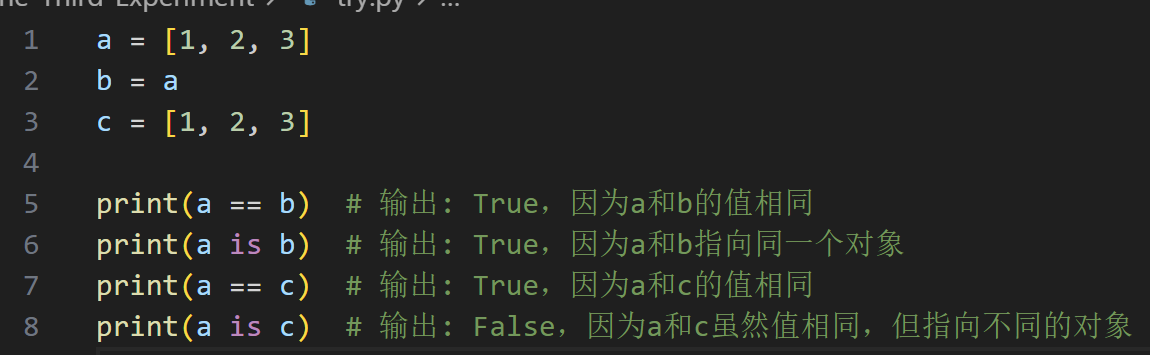
\includegraphics[scale=0.3]{pictures/7.png}
        \item \textcolor{blue}{输入输出(input(), print())}\\
        \textcolor{blue}{\textcircled{1}input()用法:括号中写出提示语句,返回值默认是字符串,如果需要特定变量类型需要加上数据转换}\\
        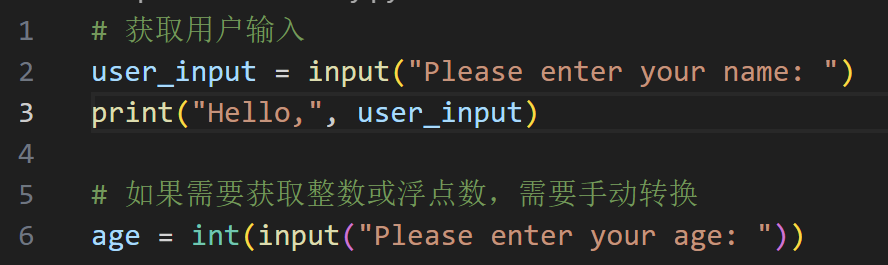
\includegraphics[scale=0.5]{pictures/8.png}\\
        \textcolor{blue}{\textcircled{2}print()用法:可以打印单个值或多个值,多个值之间可以用逗号,分隔,默认情况下,这些值会被空格分隔开}\\
        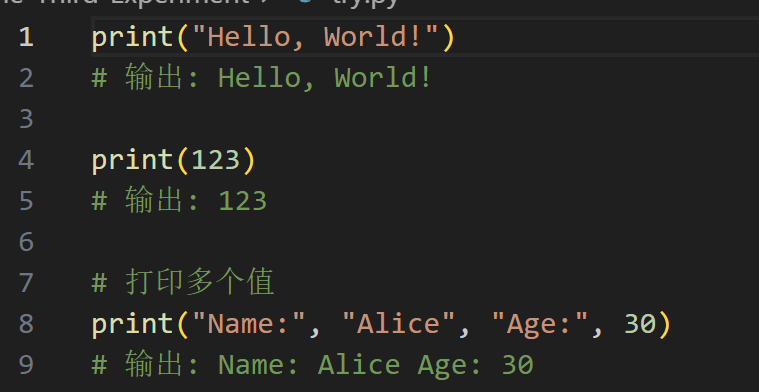
\includegraphics[scale=0.4]{pictures/9.png}\\
        \textcolor{blue}{参数}\\
        sep 参数:用于指定多个值之间的分隔符,默认为空格。\\
        end 参数:用于指定打印完所有值后添加的字符串,默认为换行符。\\
        file 参数:用于指定输出的目标文件对象,默认为sys.stdout(即标准输出)。\\
        flush 参数:布尔值,默认为False。如果为True,则强制立即写入文件(主要用于文件输出时)。\\
        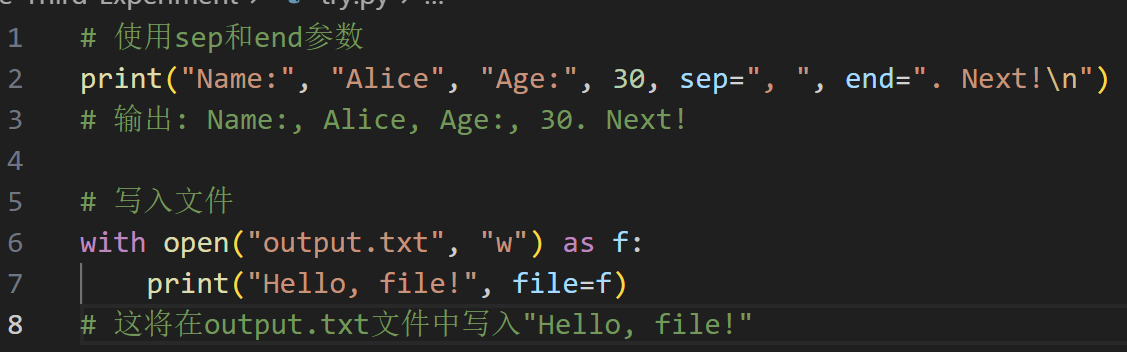
\includegraphics[scale=0.3]{pictures/10.png}
    \end{enumerate}

    \subsection{Python控制结构}
    \begin{enumerate}
        \item \textcolor{blue}{if语句及其嵌套}\\
        语法略,用法如下:\\
        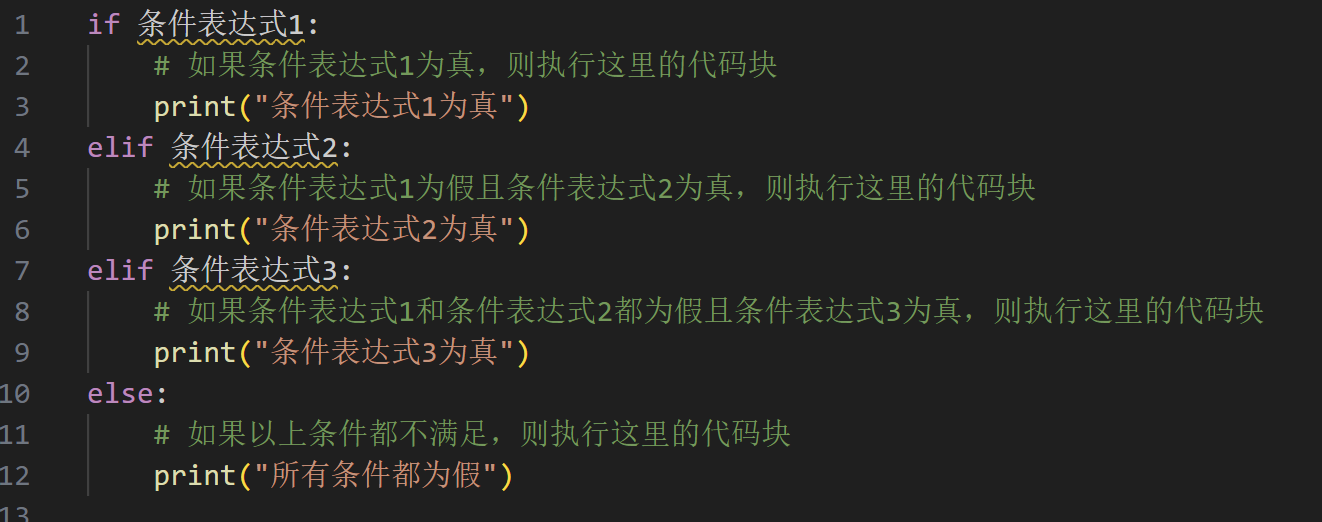
\includegraphics[scale=0.25]{pictures/11.png}\\
        \item \textcolor{blue}{for循环与while循环}\\
        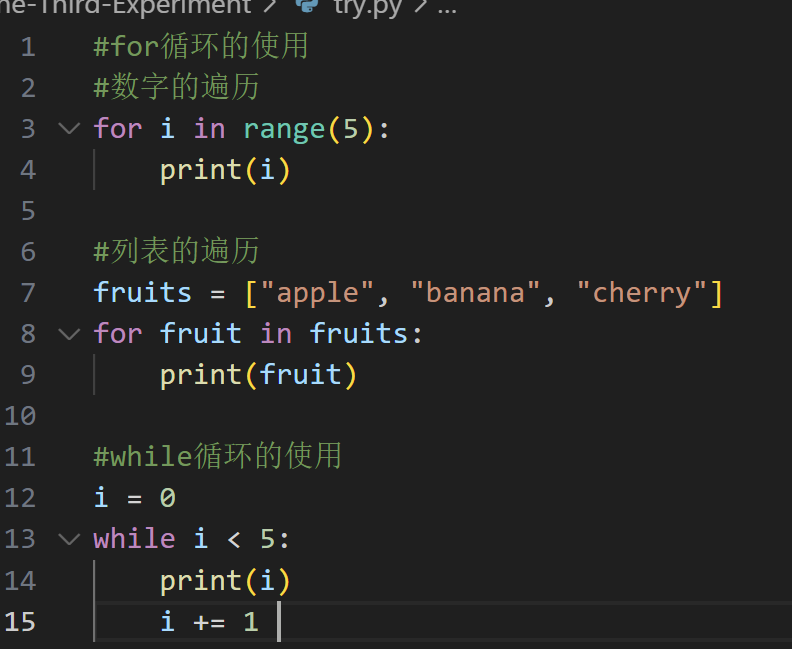
\includegraphics[scale=0.3]{pictures/12.png}\\
        \textcolor{blue}{range函数用法:}\\
        range(start, stop, step) \textcolor{red}{左开右闭}\\
        \#start(可选): 序列开始的数字,默认为0。\\
        \#stop: 序列结束的数字(但不包括此数字)。\\
        \#step(可选): 两个数字之间的间隔,默认为1。\\
        \item \textcolor{blue}{break与continue语句}\\
        \textcolor{blue}{\textcircled{1}break语句:用于立即退出当前所在的循环体}\\
        \textcolor{blue}{\textcircled{2}coontinue语句:用于跳过当前循环迭代中continue语句之后的代码,并继续下一次循环迭代}\\
    \end{enumerate}

    \subsection{Python视觉应用}
    \begin{enumerate}
        \item \textcolor{blue}{open():函数用于创建PIL 图像对象}\\
        \item \textcolor{blue}{save():方法用于保存图像到具有指定文件名的文件}\\[8pt]
        \textcolor{red}{例:将一个jpg文件转换成png格式}\\
        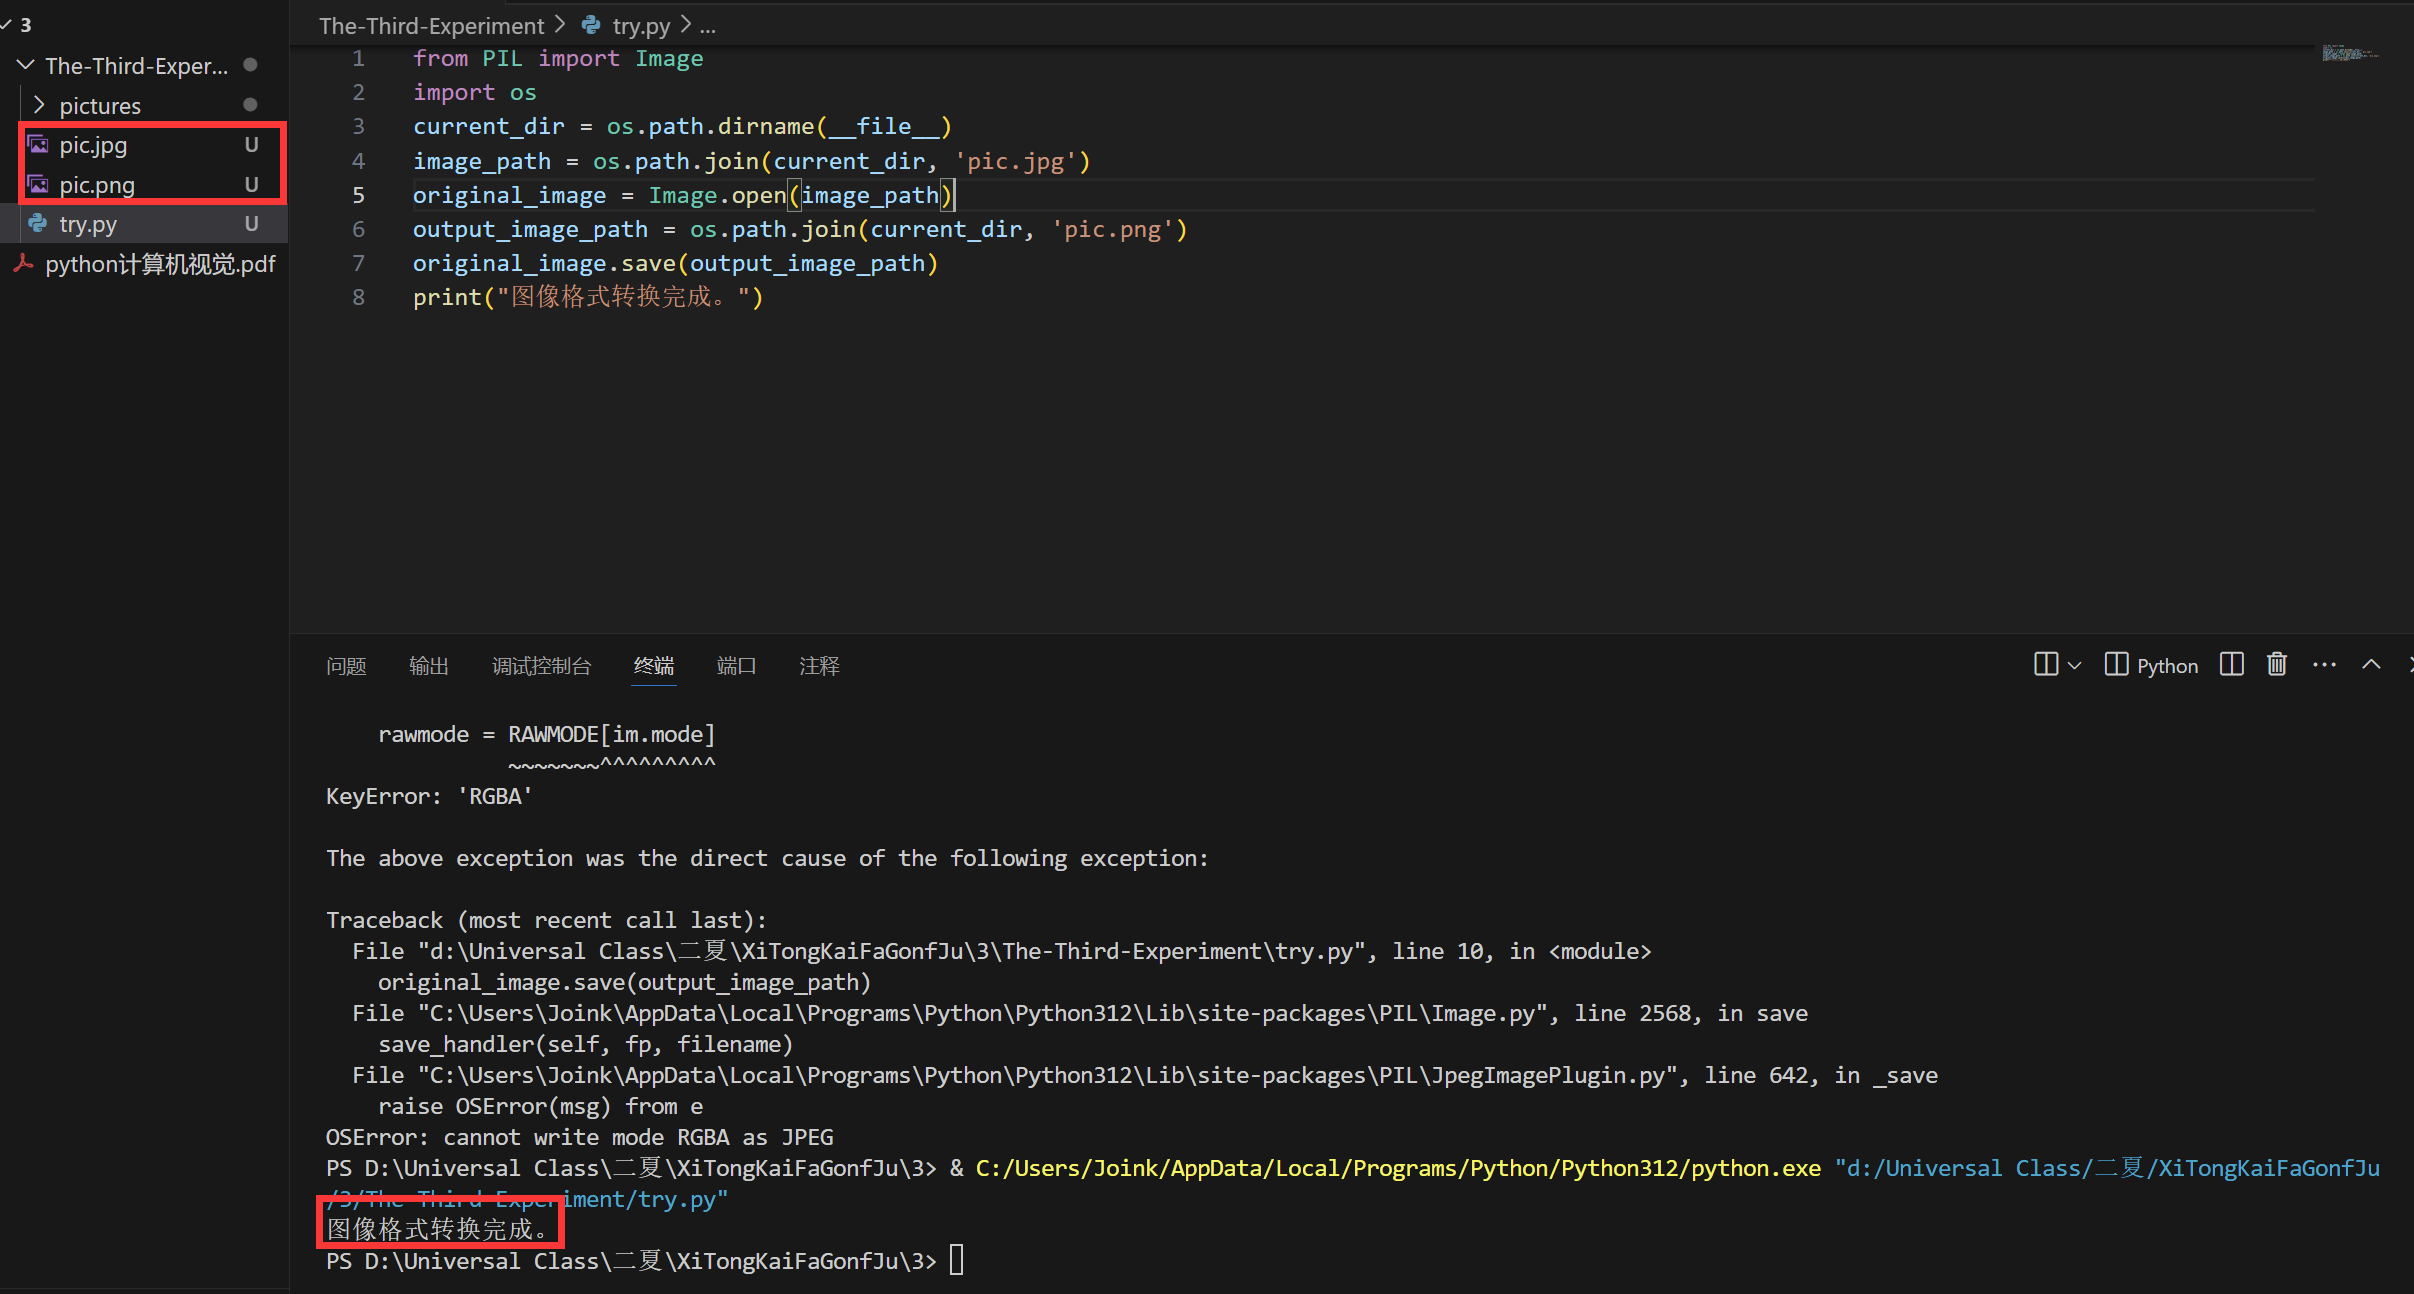
\includegraphics[scale=0.25]{pictures/13.png}\\
        \item \textcolor{blue}{crop():从一幅图像中裁剪指定区域}\\
        \item \textcolor{blue}{paste():粘贴图像到指定位置}\\
        \textcolor{red}{例:将一个图片的一角复制粘贴到原图中间}\\
        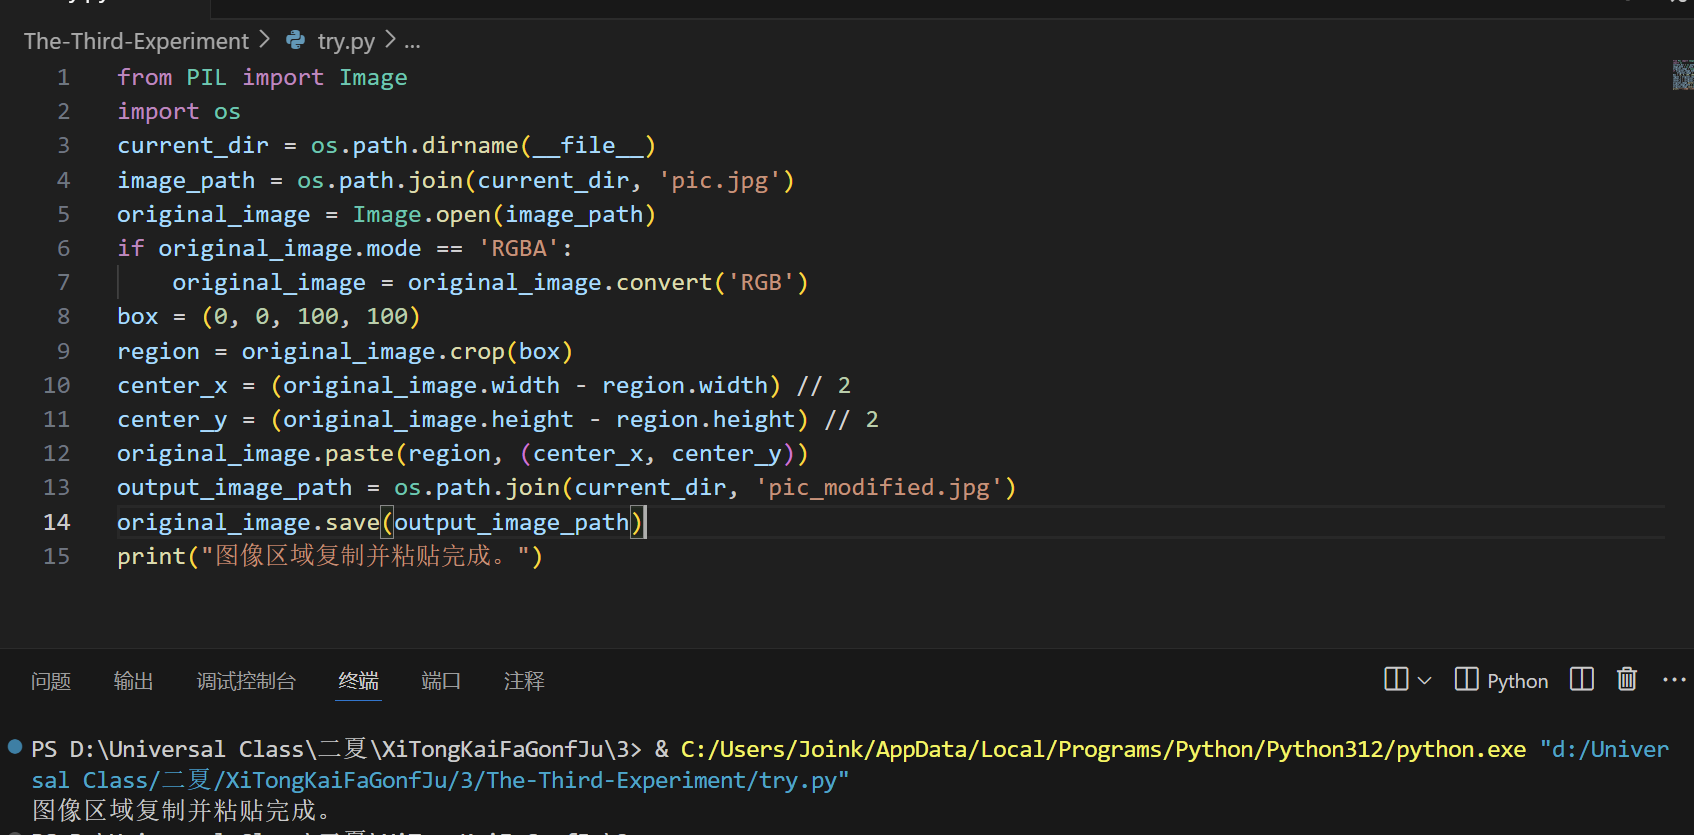
\includegraphics[scale=0.25]{pictures/14.png}\\
        生成图如下:\\
        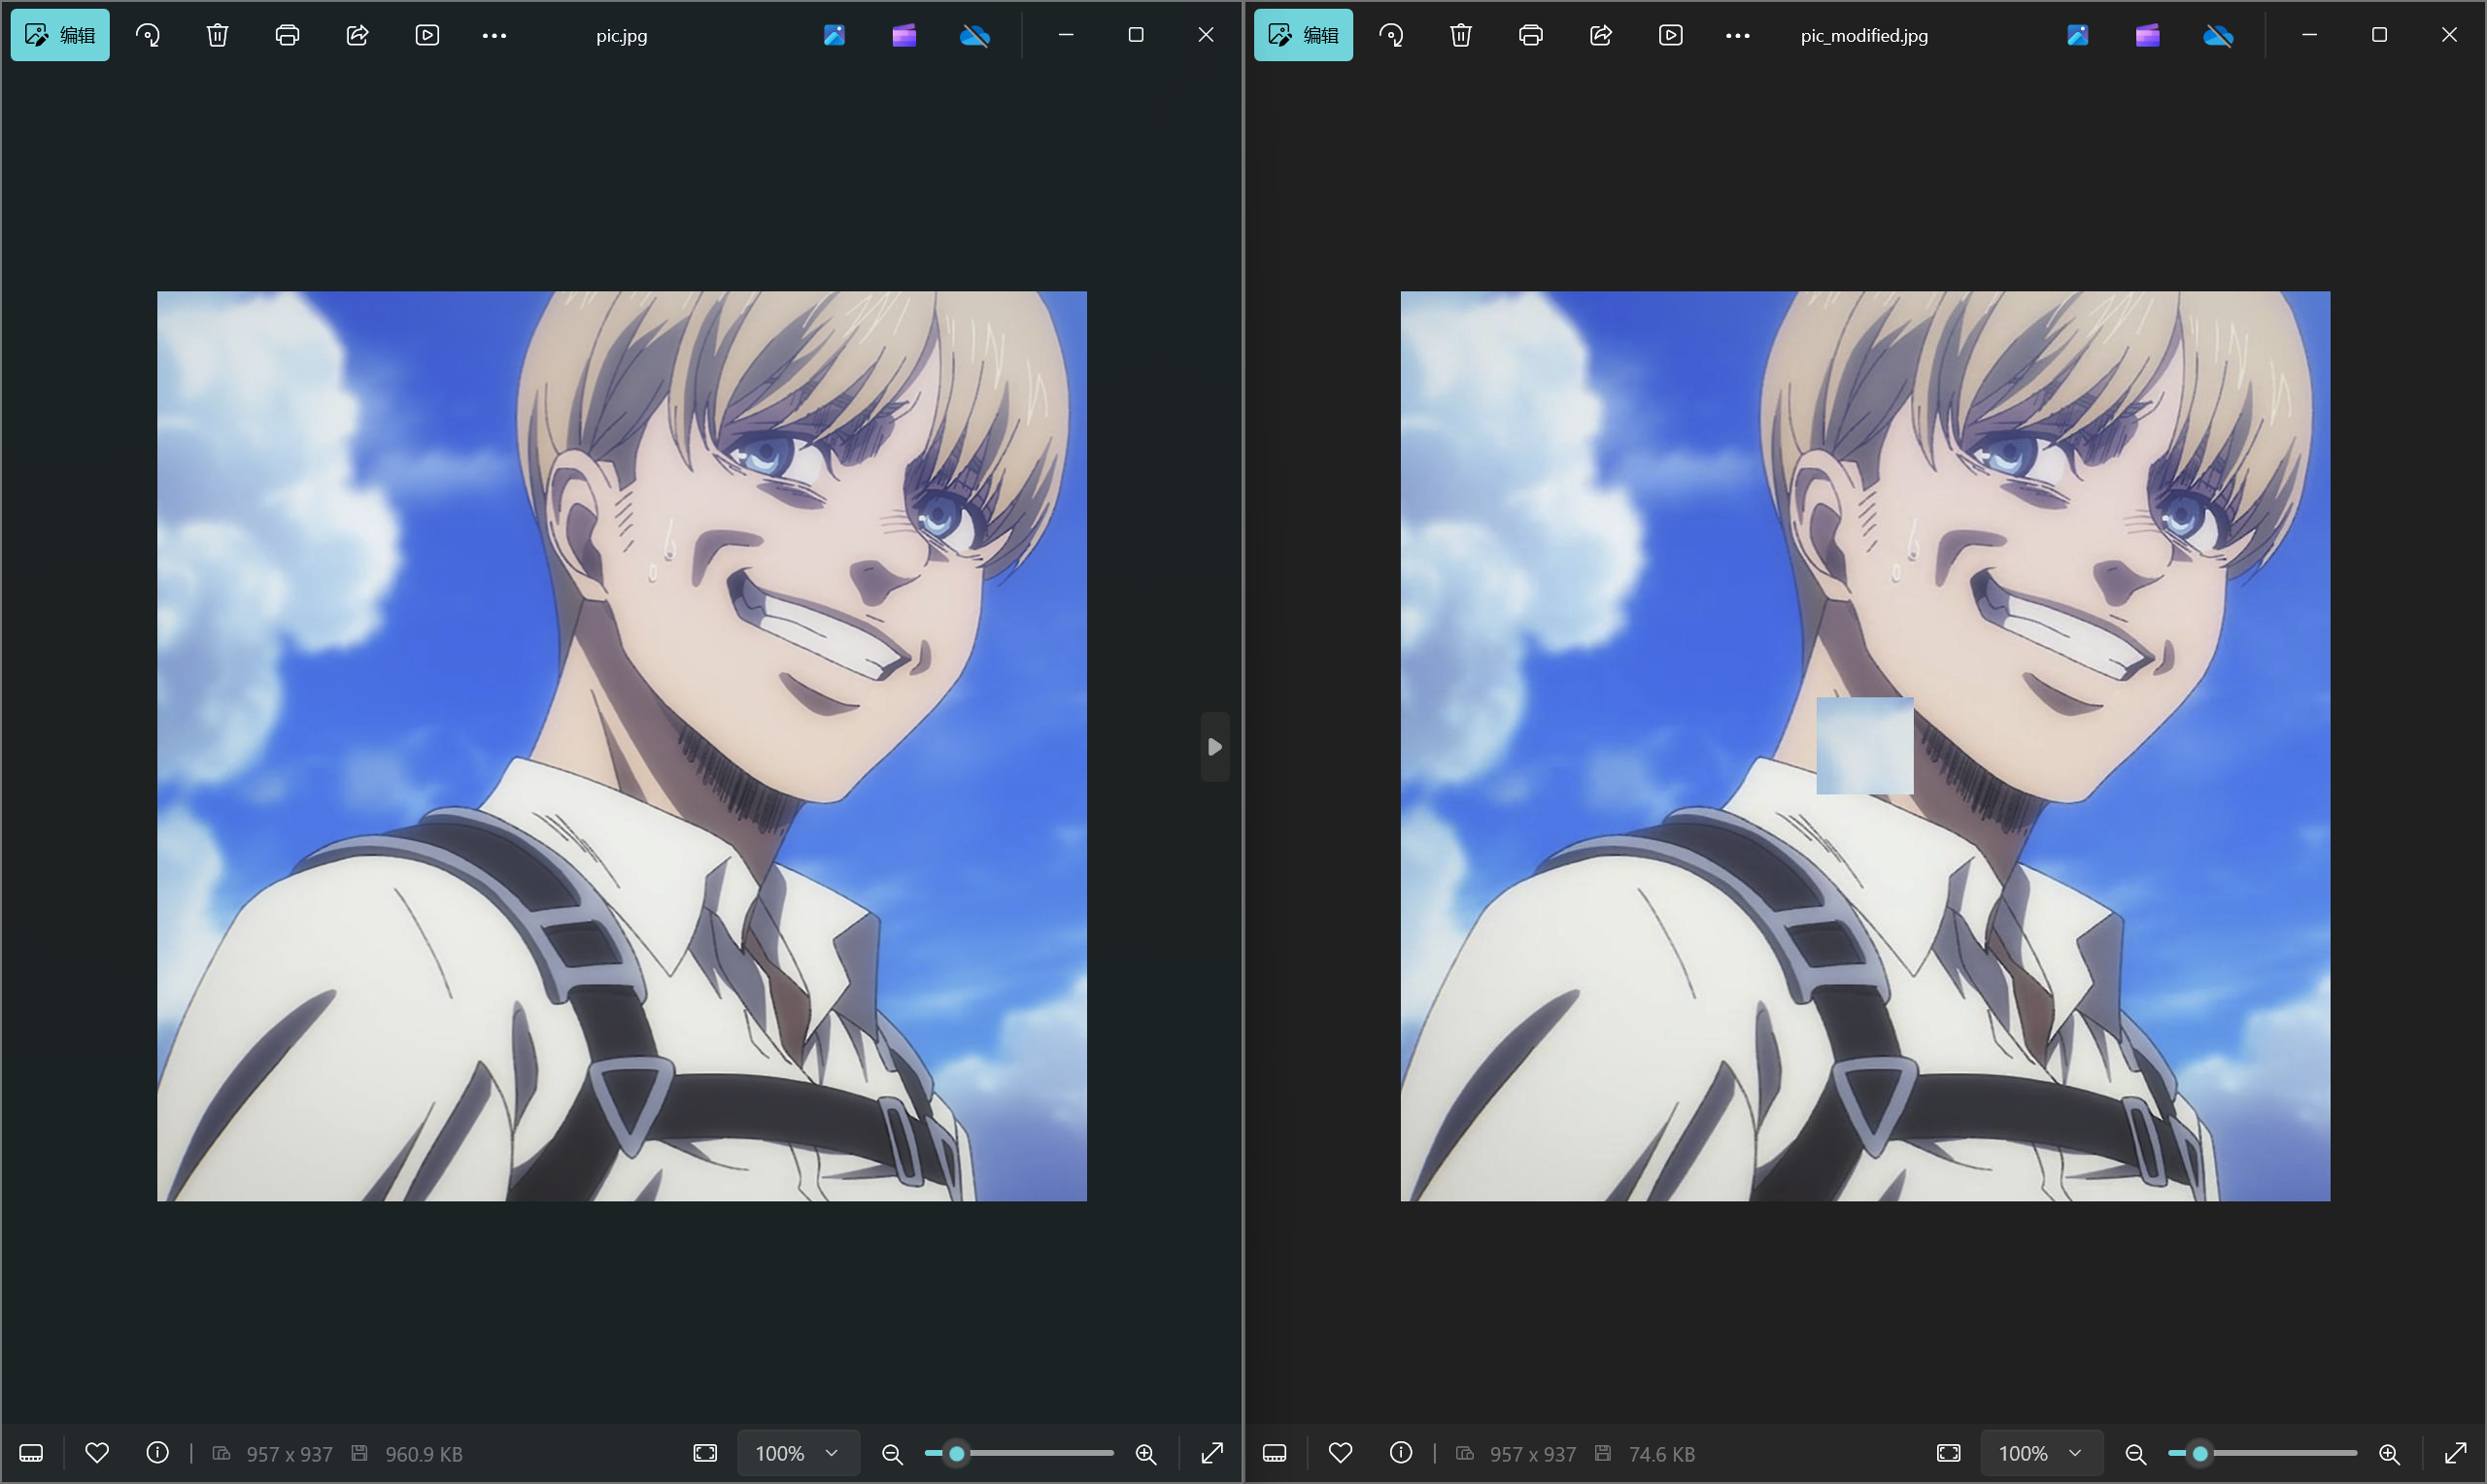
\includegraphics[scale=0.15]{pictures/14_2.png}\\
        \item \textcolor{blue}{resize():用元祖指定图片的大小}\\
        \item \textcolor{blue}{rotate():用角度指定图片的旋转}\\
        \textcolor{red}{例:将原图缩小并旋转90度}\\
        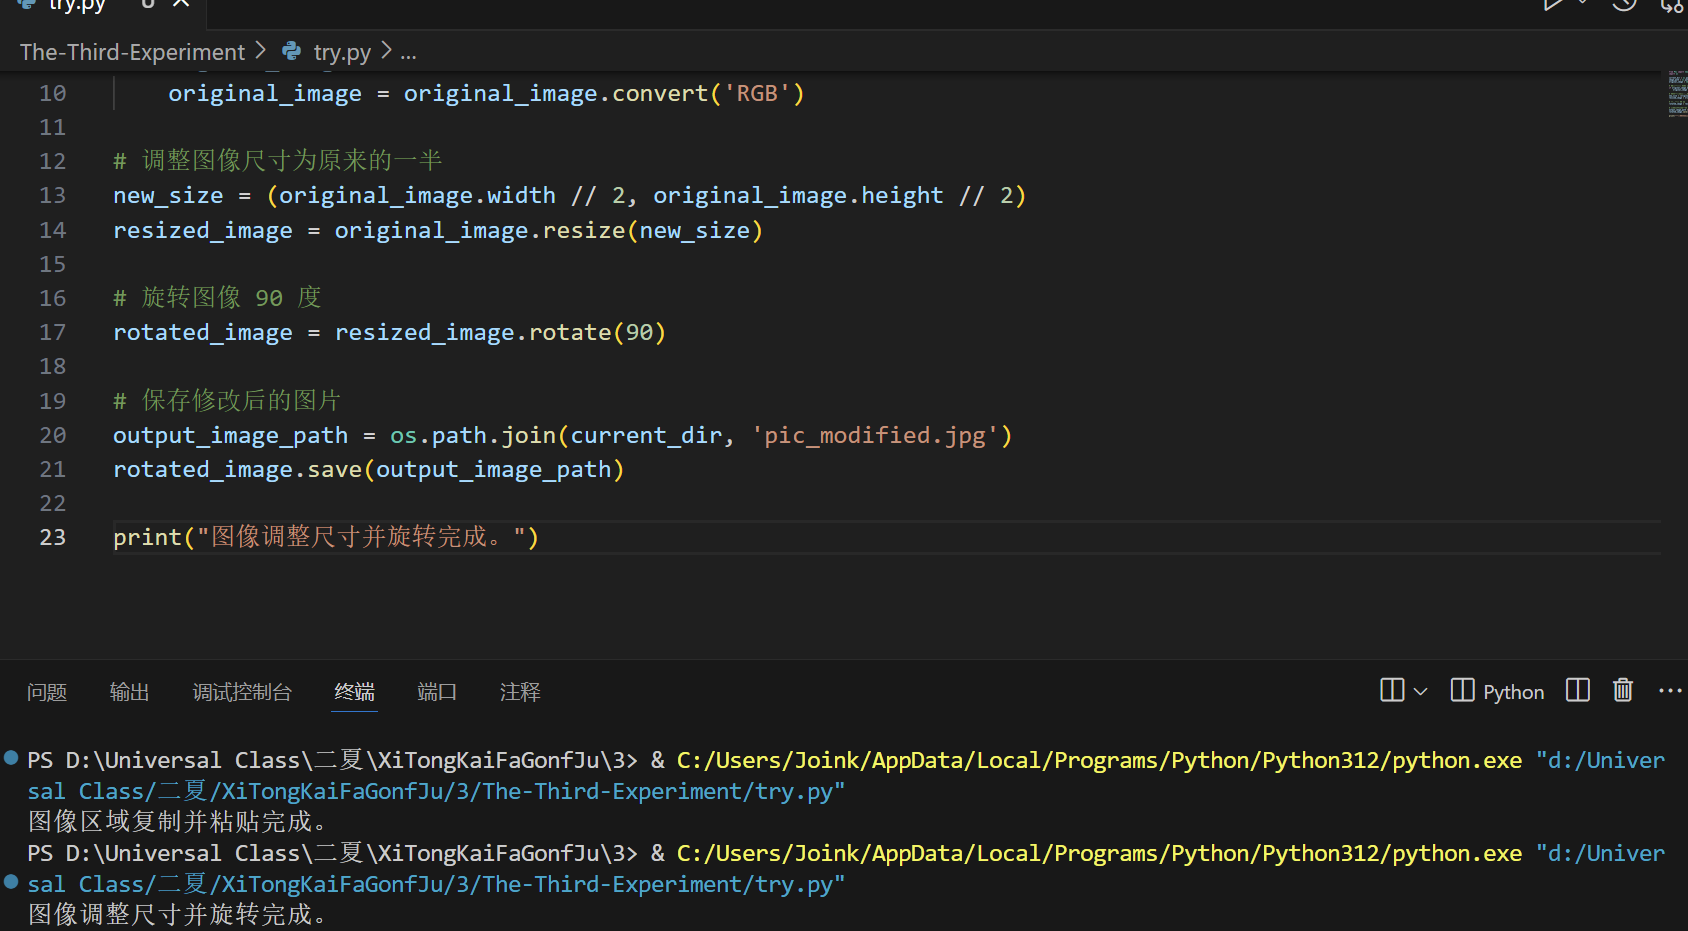
\includegraphics[scale=0.25]{pictures/15.png}
        生成图如下:\\
        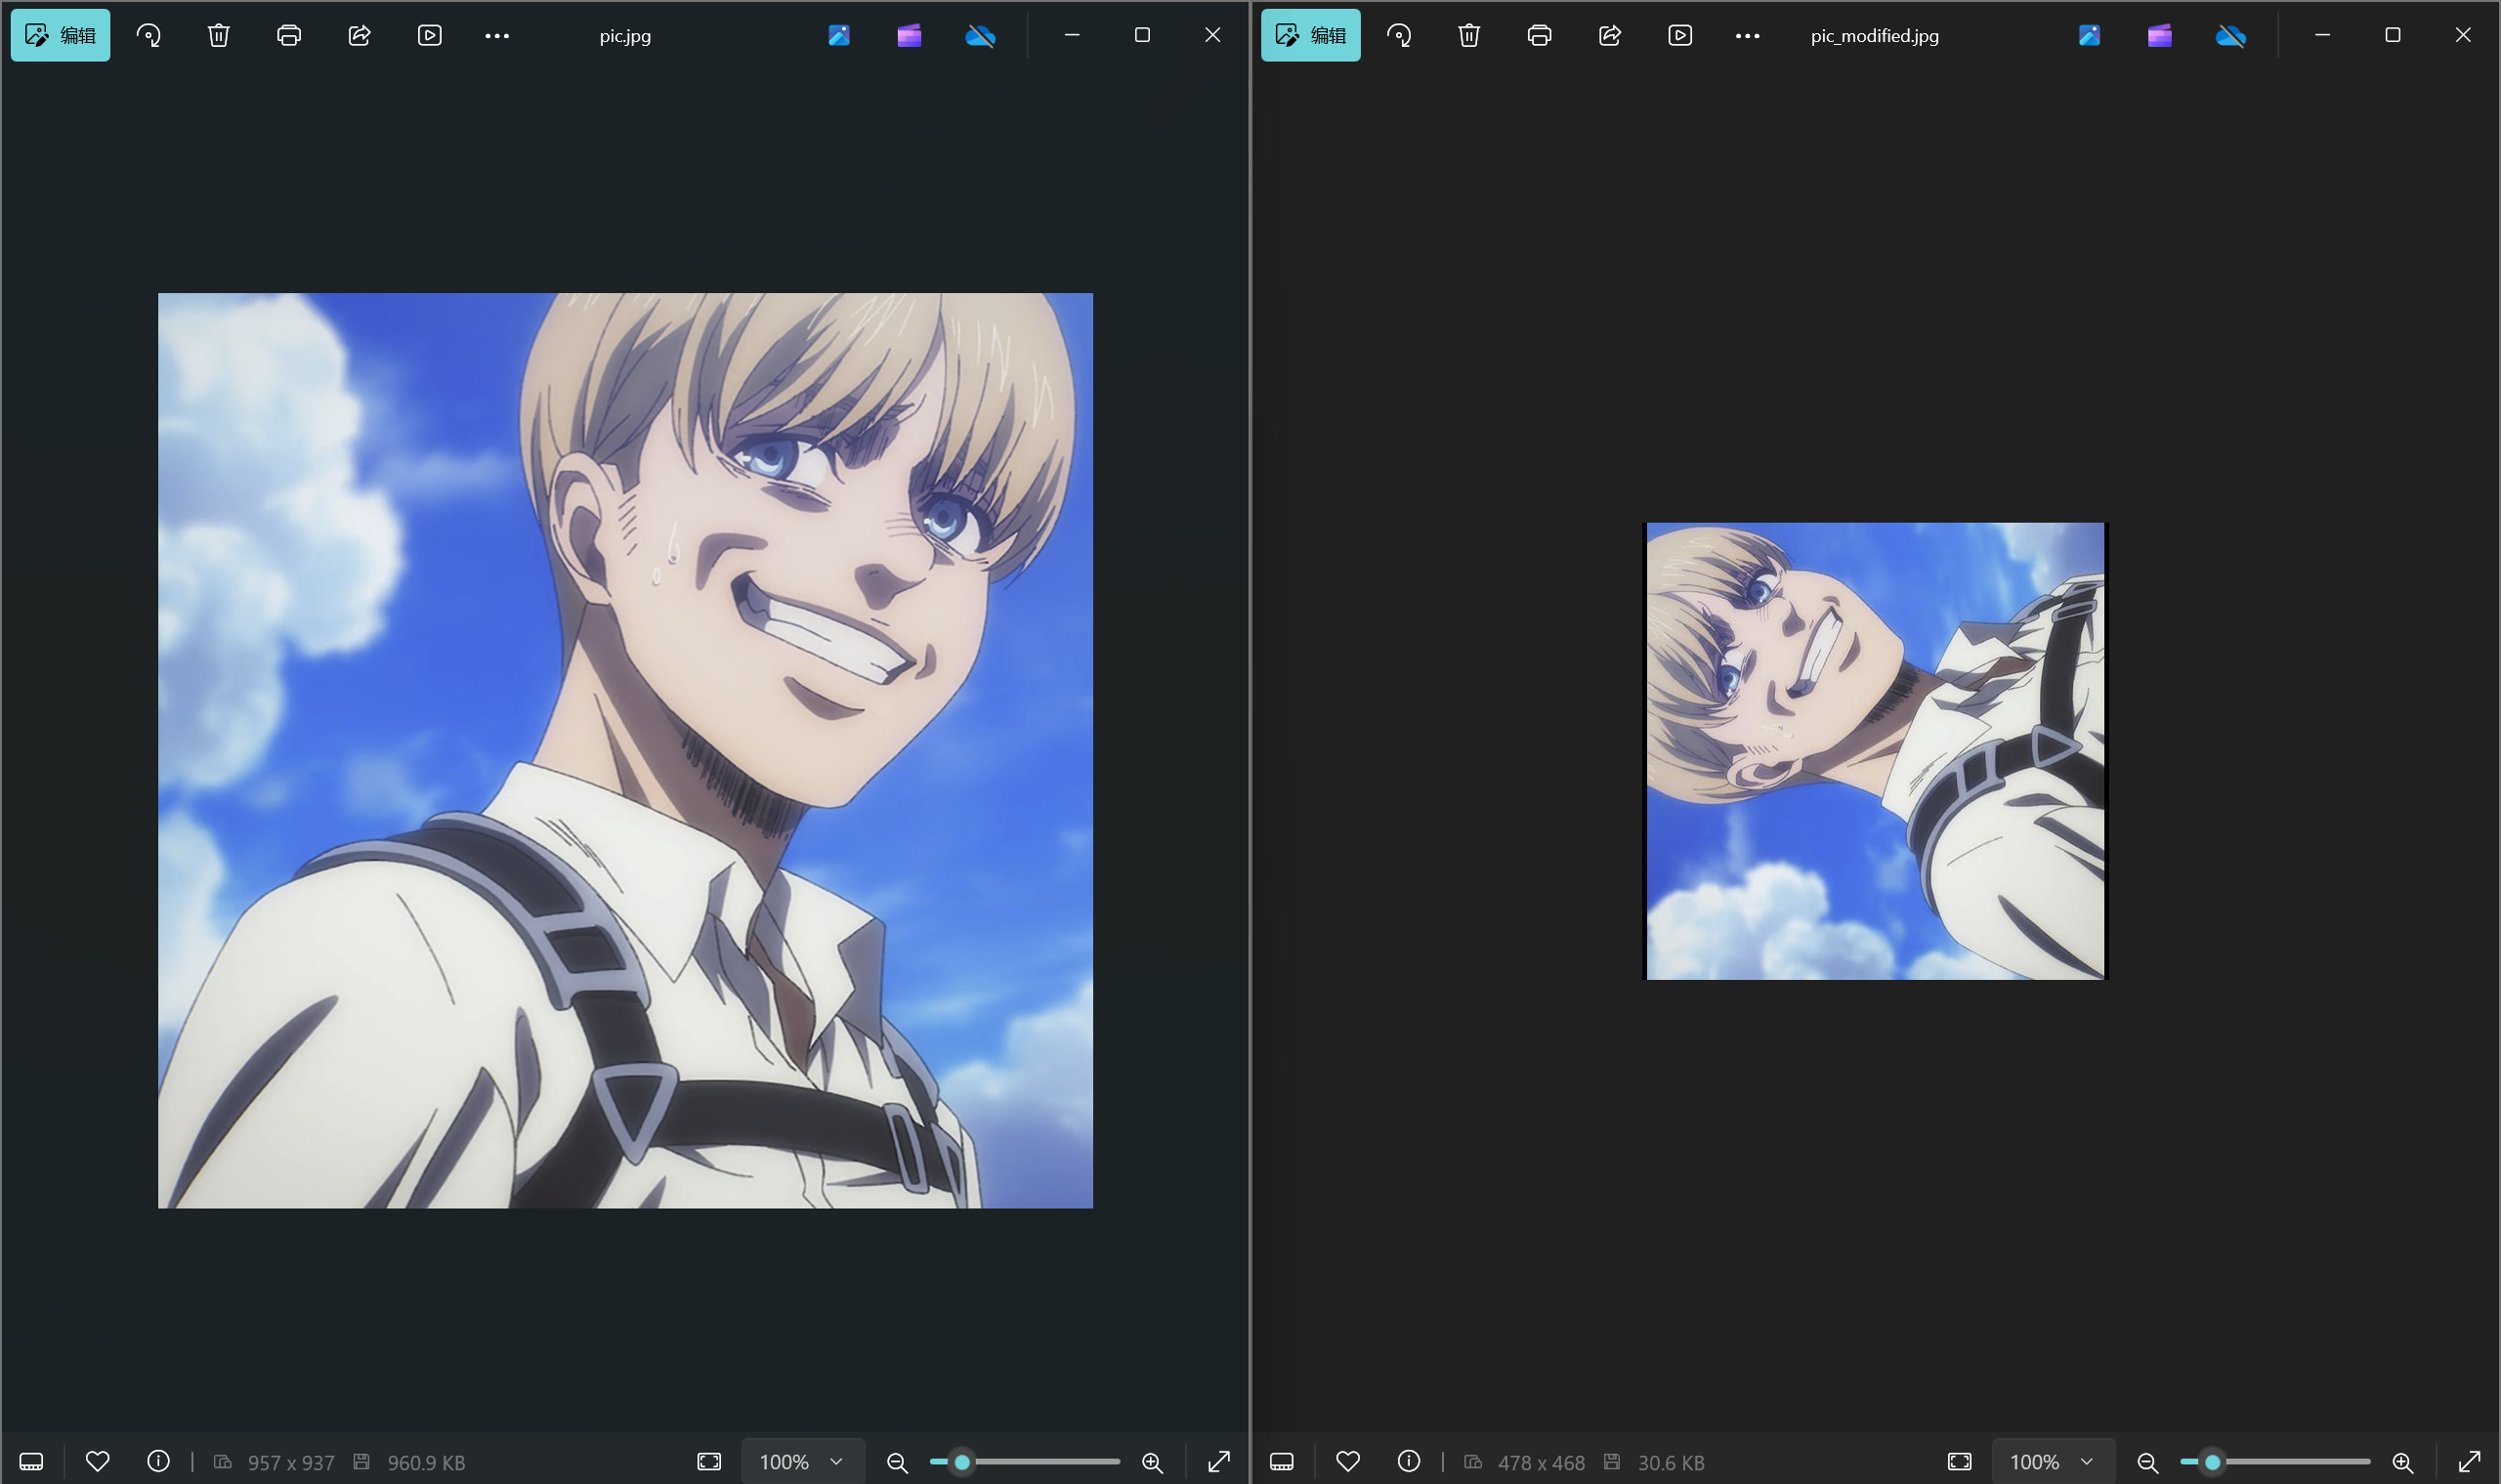
\includegraphics[scale=0.15]{pictures/15_2.png}\\
        \item \textcolor{blue}{plot(x,y):绘制大小为x和y数据点的折线图}\\
        \item \textcolor{blue}{xlabel(角标):设置图标x轴角标}\\
        \item \textcolor{blue}{ylabel(角标):设置图标y轴角标}\\
        \item \textcolor{blue}{title(标题):设置图标标题}\\
        \item \textcolor{blue}{grid(true/false):设置是否启用网格线}\\
        \item \textcolor{blue}{imshow(图片地址,图片信息,aspect=显示范围,alpha=透明度):在图表中显示图像 img,设置图像的显示范围和透明度。}\\
        \textcolor{red}{例:将原图放在坐标轴中}\\
        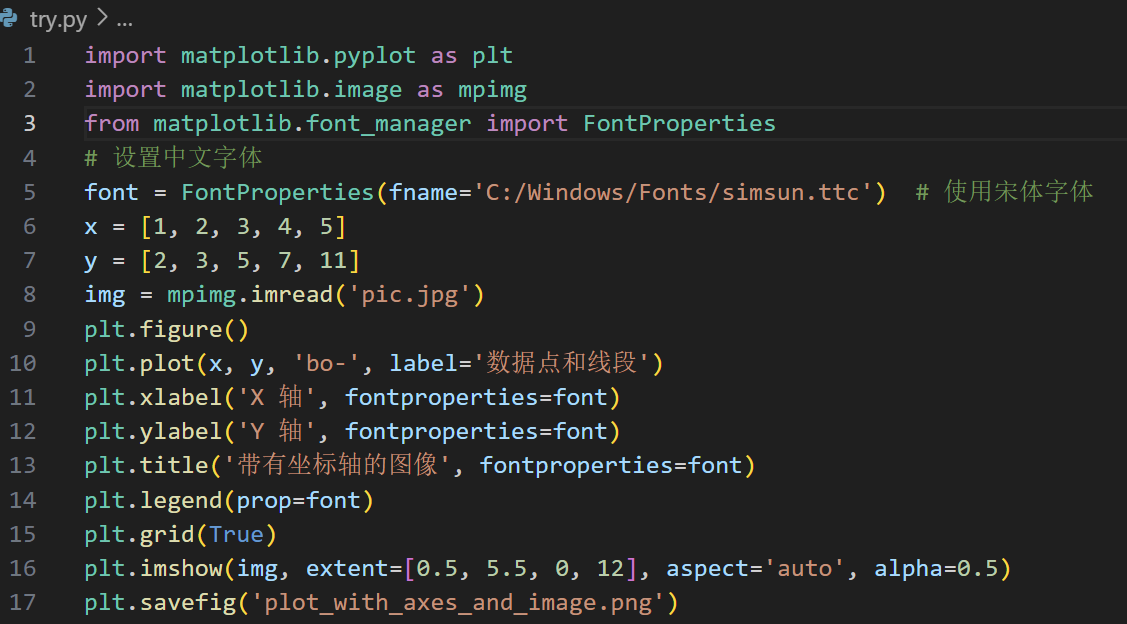
\includegraphics[scale=0.25]{pictures/16.png}\\
        生成图如下:\\
        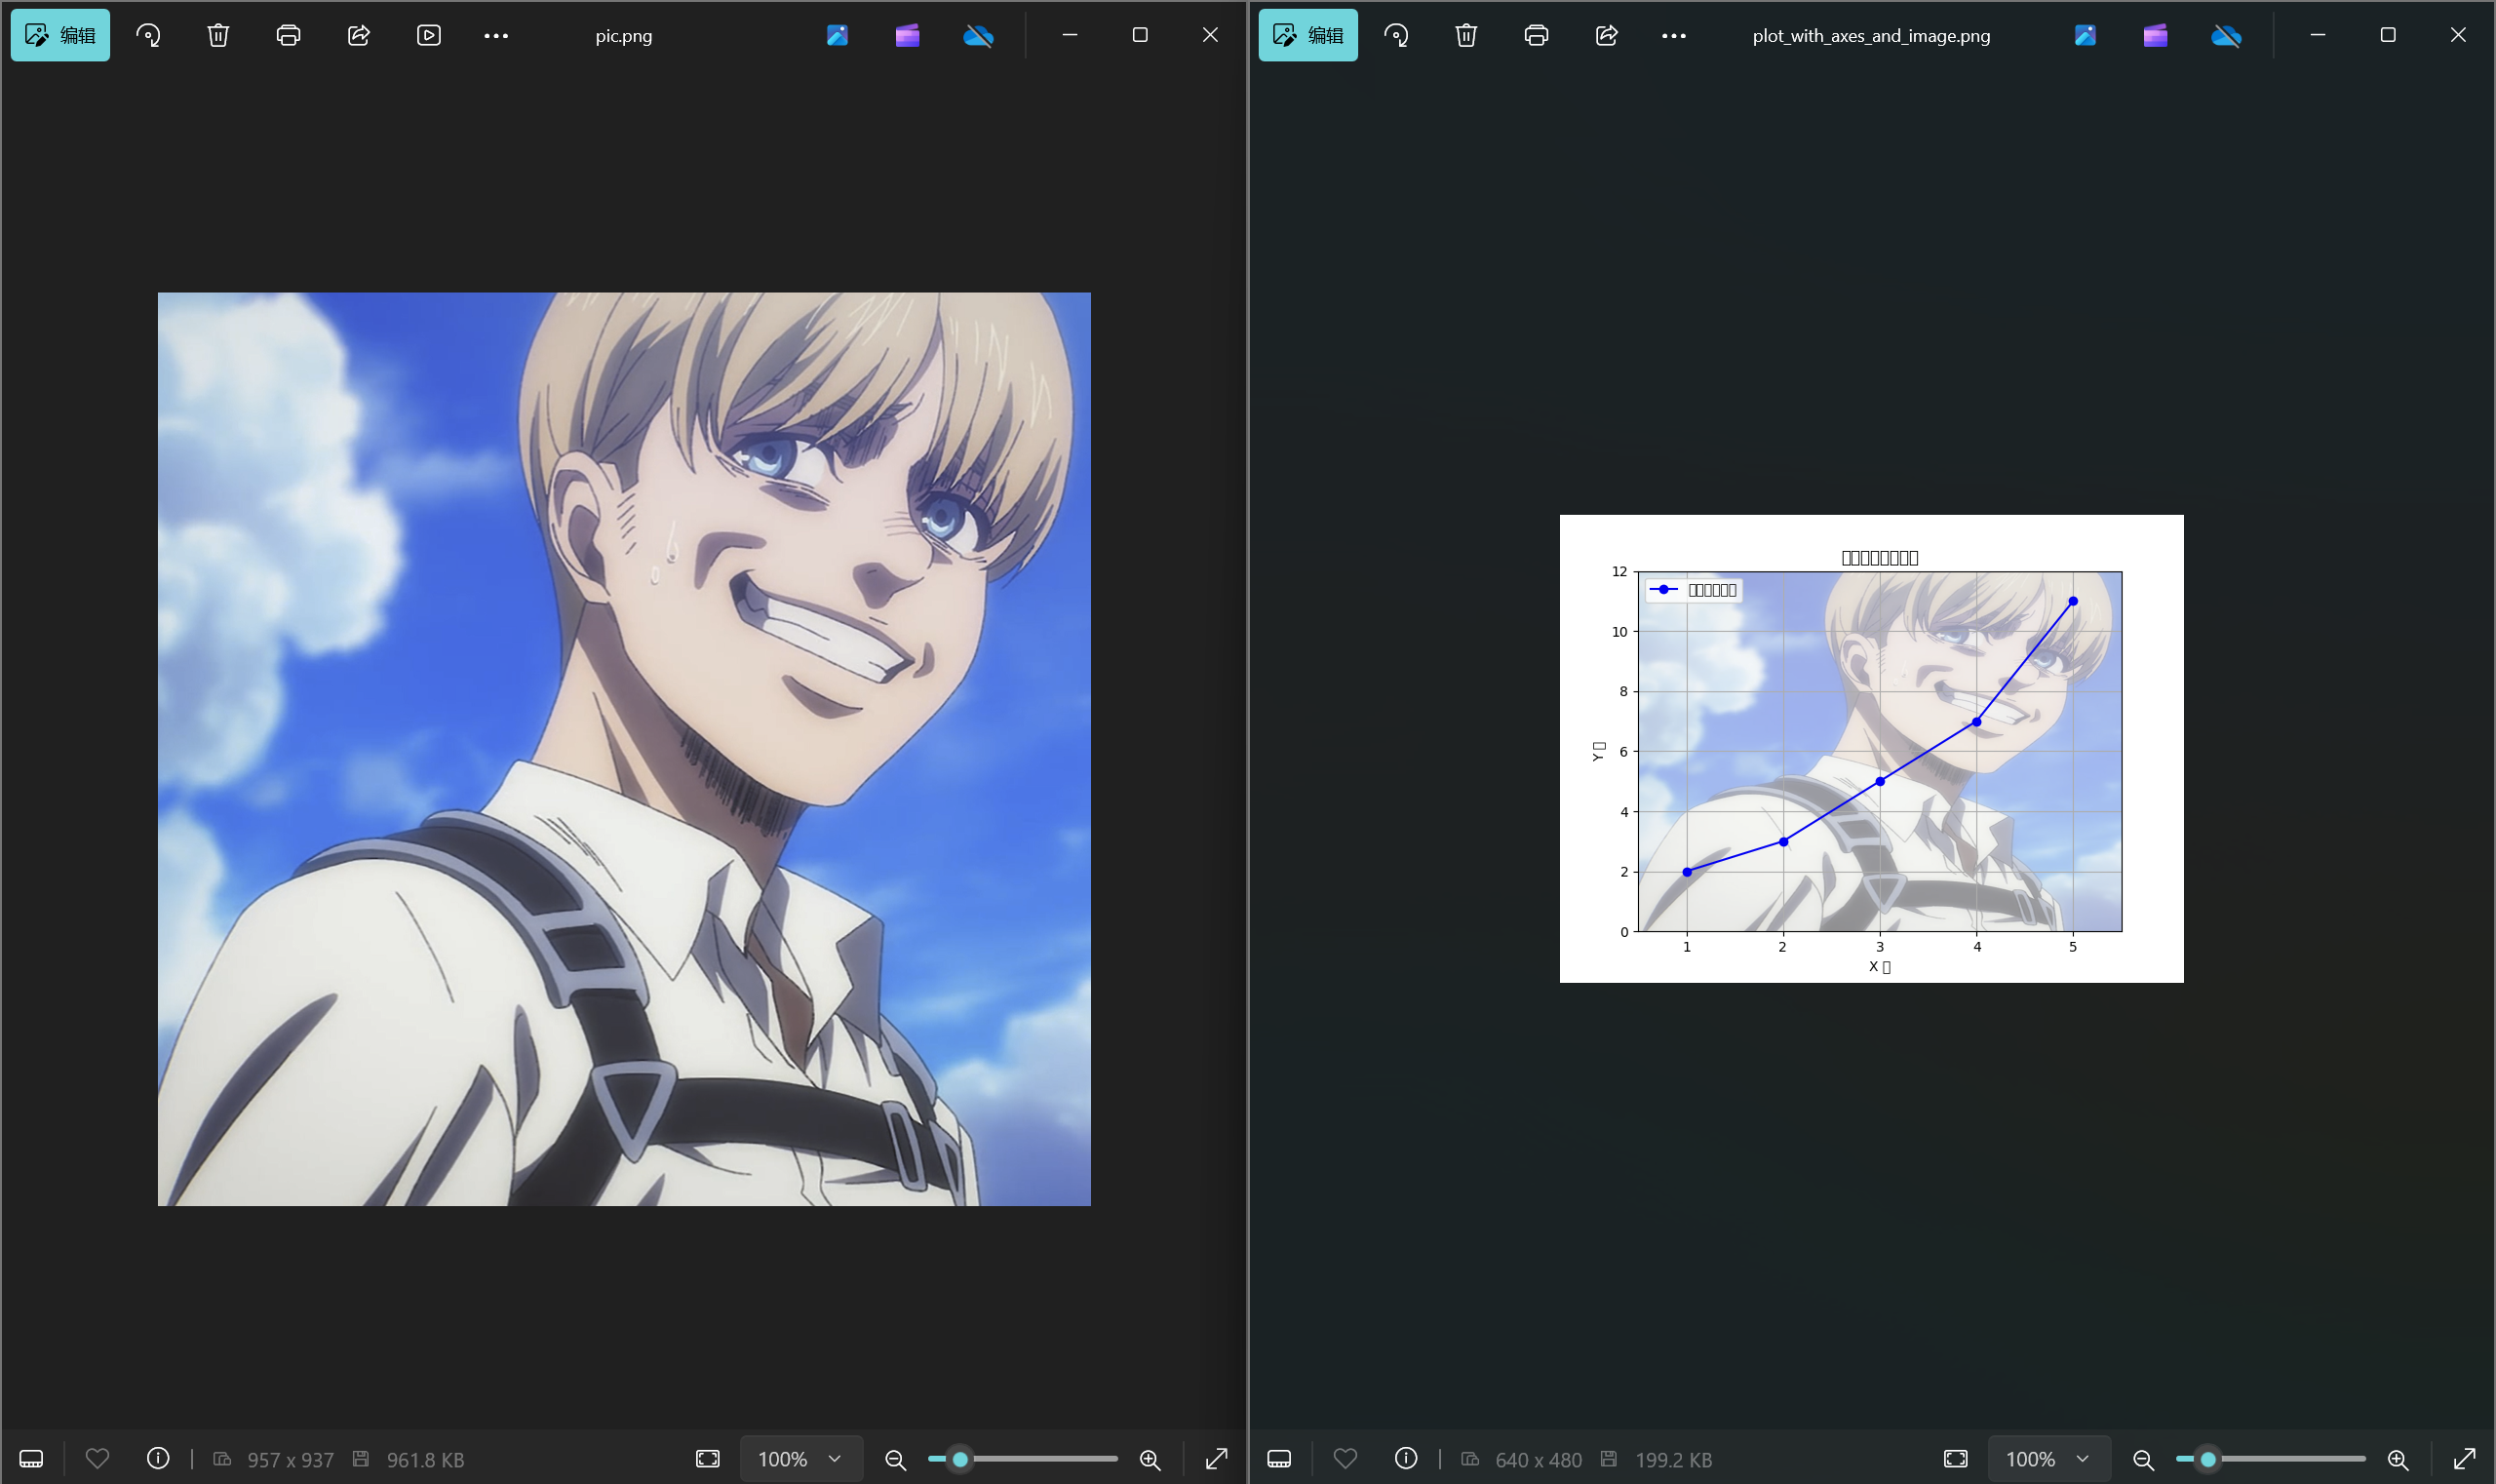
\includegraphics[scale=0.15]{pictures/16_2.png}\\
        \textcolor{red}{例:使用ROF模型对合成图像去噪}\\
        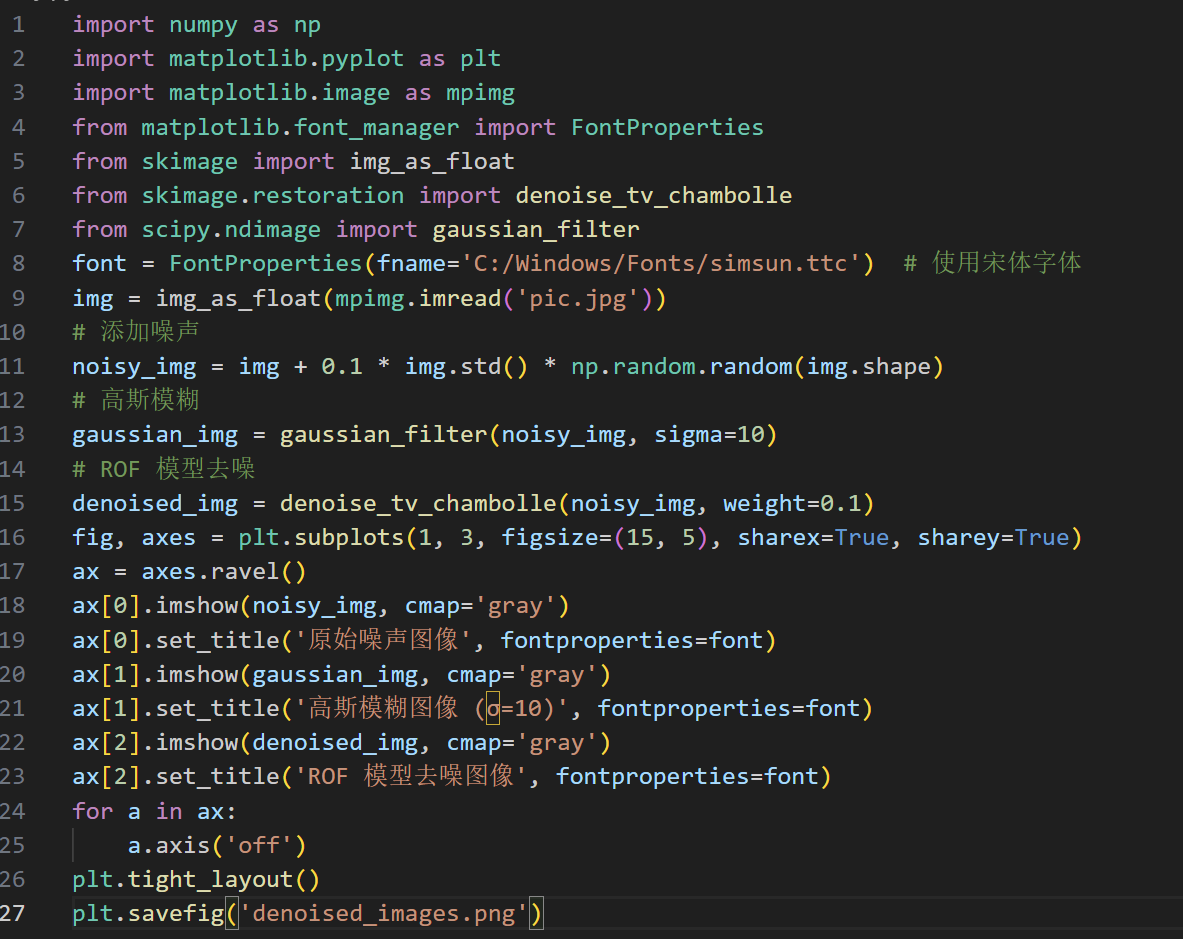
\includegraphics[scale=0.35]{pictures/17.png}\\
        生成图如下:\\
        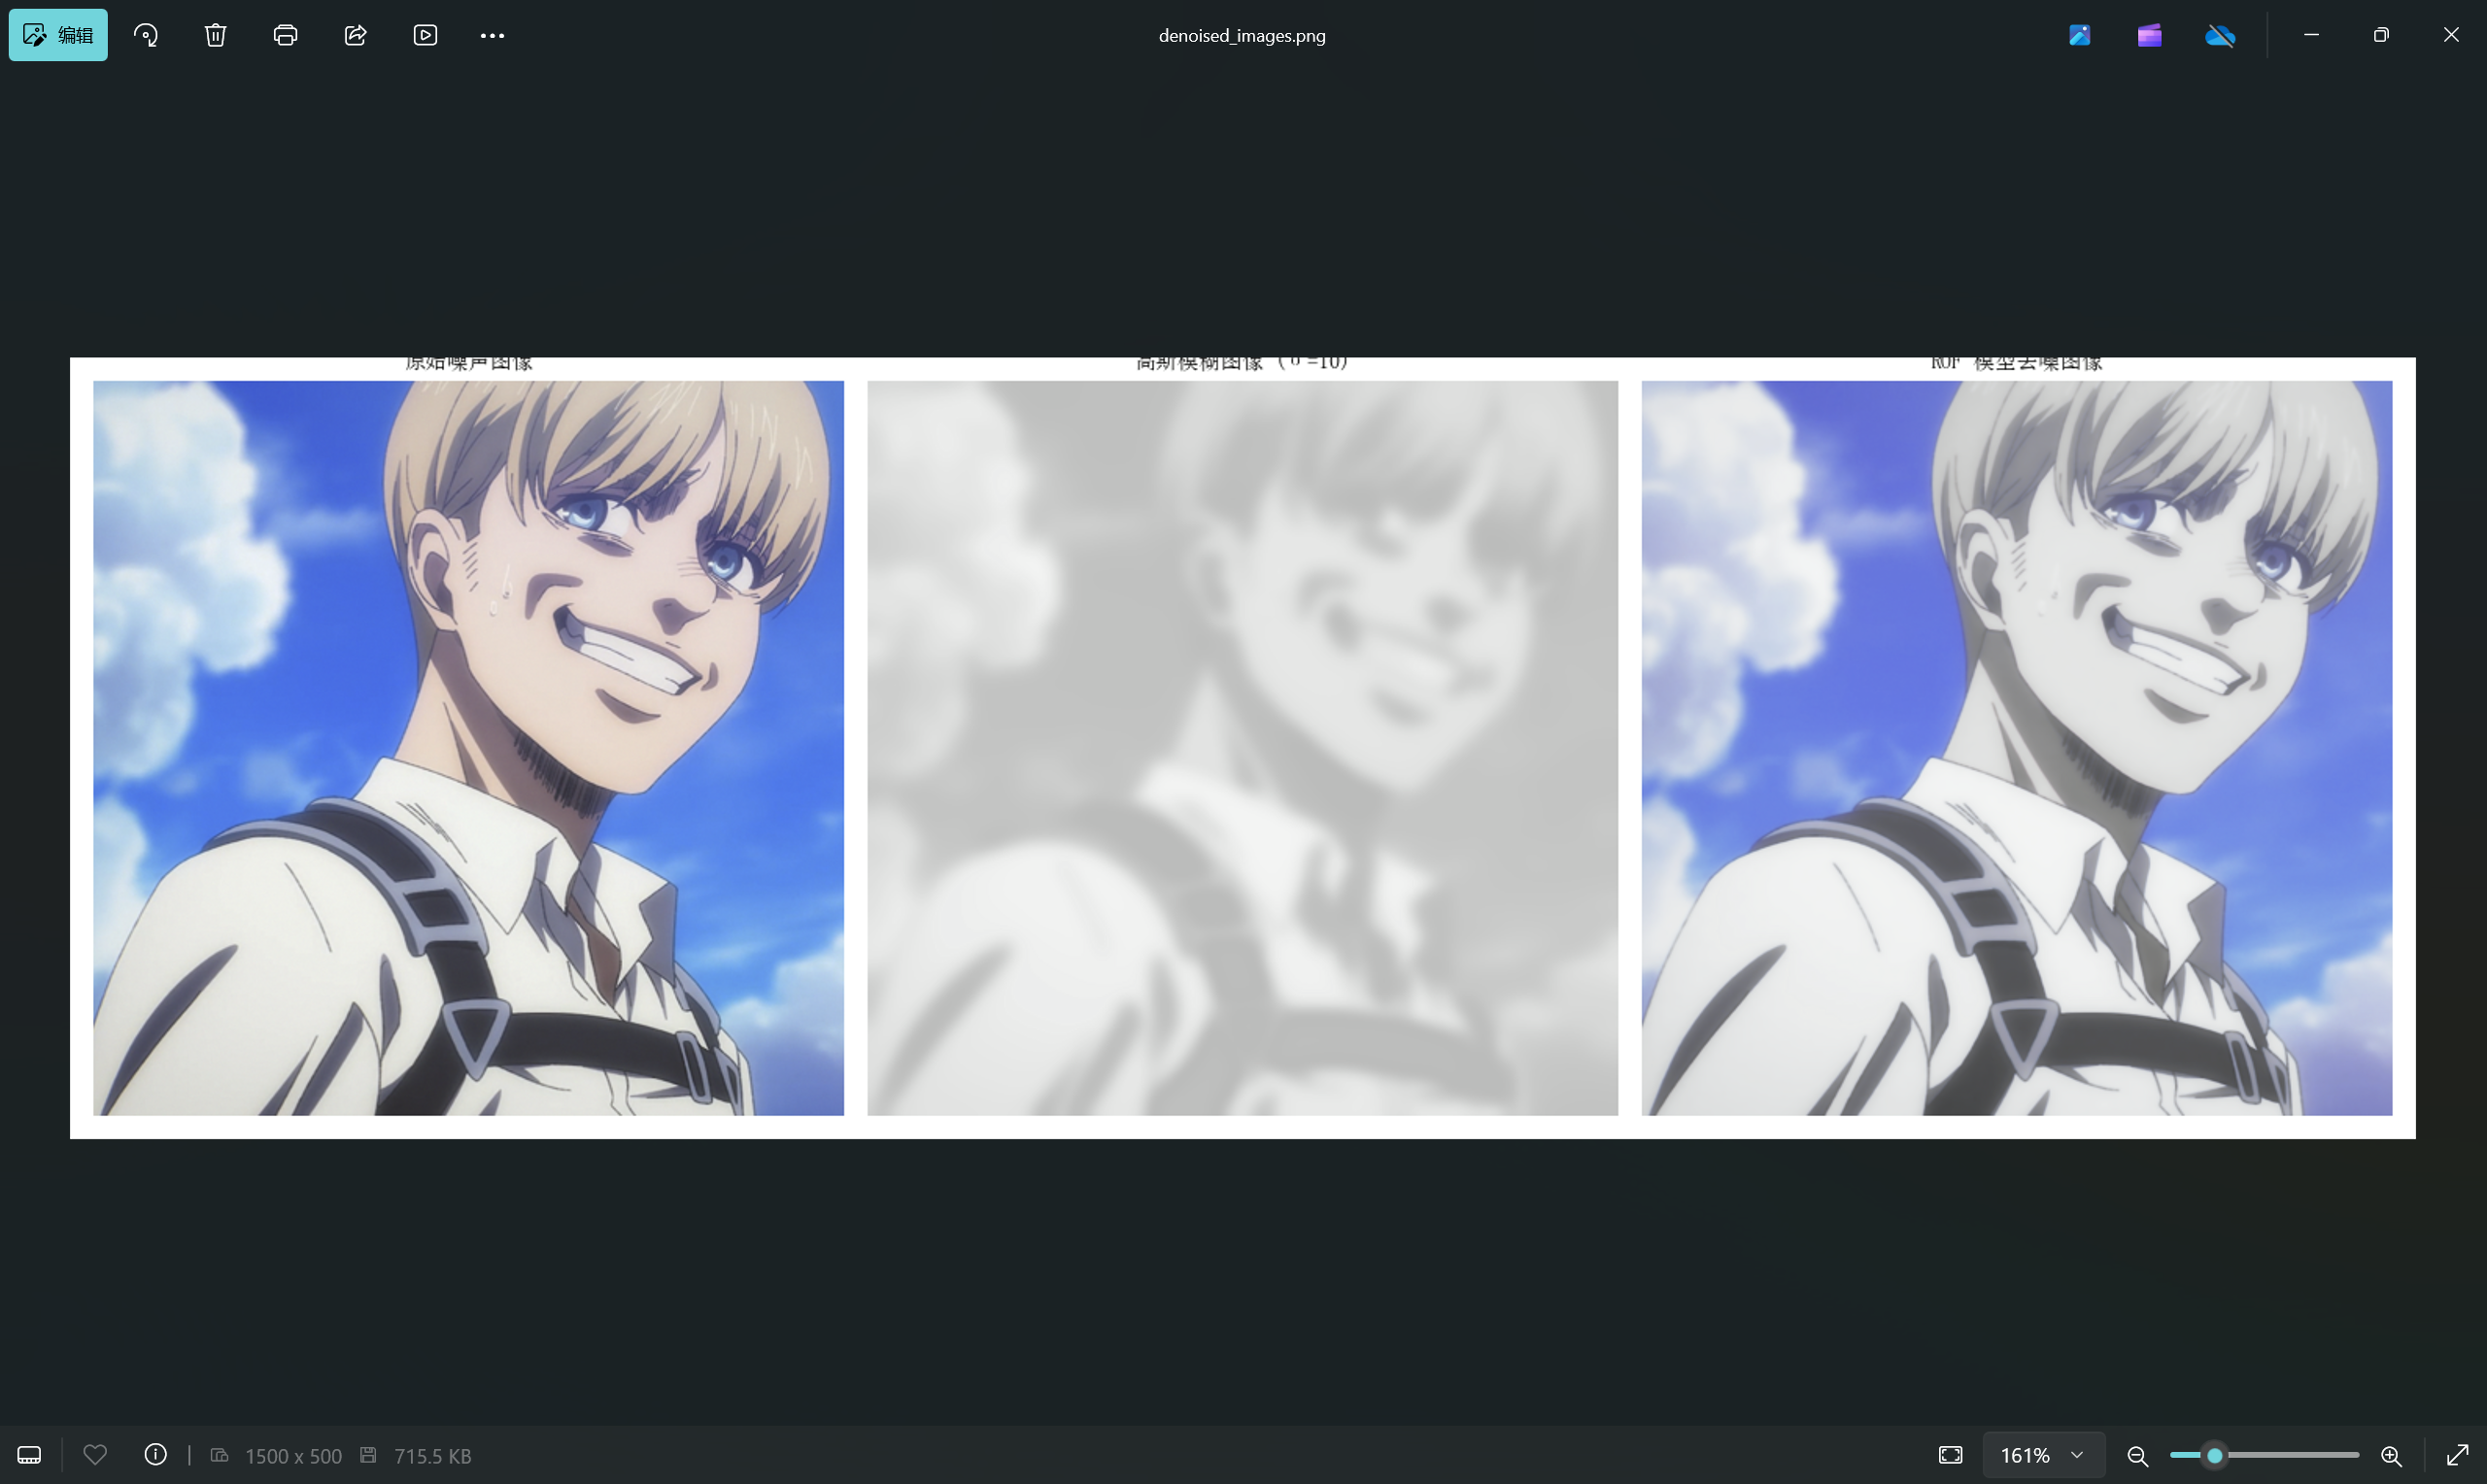
\includegraphics[scale=0.15]{pictures/17_2.png}\\
        中间重要语句的注释如下:\\
        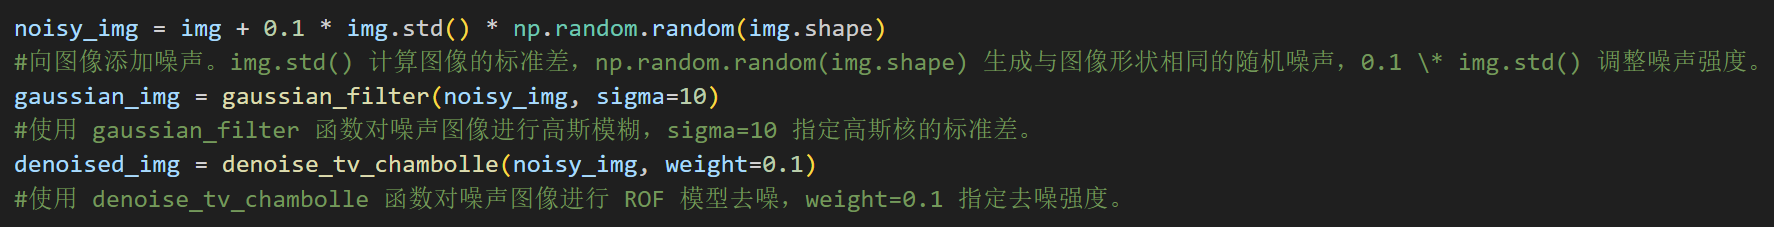
\includegraphics[scale=0.25]{pictures/18.png}
    \end{enumerate}
    
    \NoBgThispage
    \section{实验感悟}
    通过本次实验,我对Python编程有了更深入的理解和实践体验。实验分为两个主要部分:Python基础和Python视觉应用。

    \subsection{Python基础}
    在Python基础部分,我学习了Python的基本数据类型、控制结构以及函数与模块的使用,具体为:变量定义与数据类型、运算符与表达式、输入输出(input(), print())、if语句及其嵌套、for循环与while循环、break与continue语句

    \subsection{Python视觉}
    在Python视觉应用部分,我学习了如何使用Python进行图像处理。通过使用PIL库和matplotlib库,练习图像的读取、保存、裁剪、粘贴、缩放、旋转等基本操作。同时,通过对图像添加噪声、高斯模糊以及使用ROF模型去噪的实践,对图像处理的基本原理有了更深入的理解。

    \subsection{}
    本次实验不仅让我掌握了Python的基础知识和图像处理技术,还培养了我解决实际问题的能力。在实验过程中,我遇到了PIP安装失败,Python环境路径没有配置,Python环境路径重复,无法显示中文等问题,但通过查阅资料和不断尝试,最终解决了这些问题。这让我深刻体会到编程学习中实践的重要性。通过不断地动手操作和解决问题,我不仅加深了对理论知识的理解,也提升了自己的编程技能和逻辑思维能力。
    
\end{document}